\subsection{Course of the Disease}
\label{sub:course_of_disease}

The following medical parameters describing the progression of the disease are taken from systematic reviews (e.g. \cite{He2020}). After an infection occurs, the disease progresses in the way depicted in Figure~\ref{fig:course_of_disease}.

\begin{figure}[!tp]
    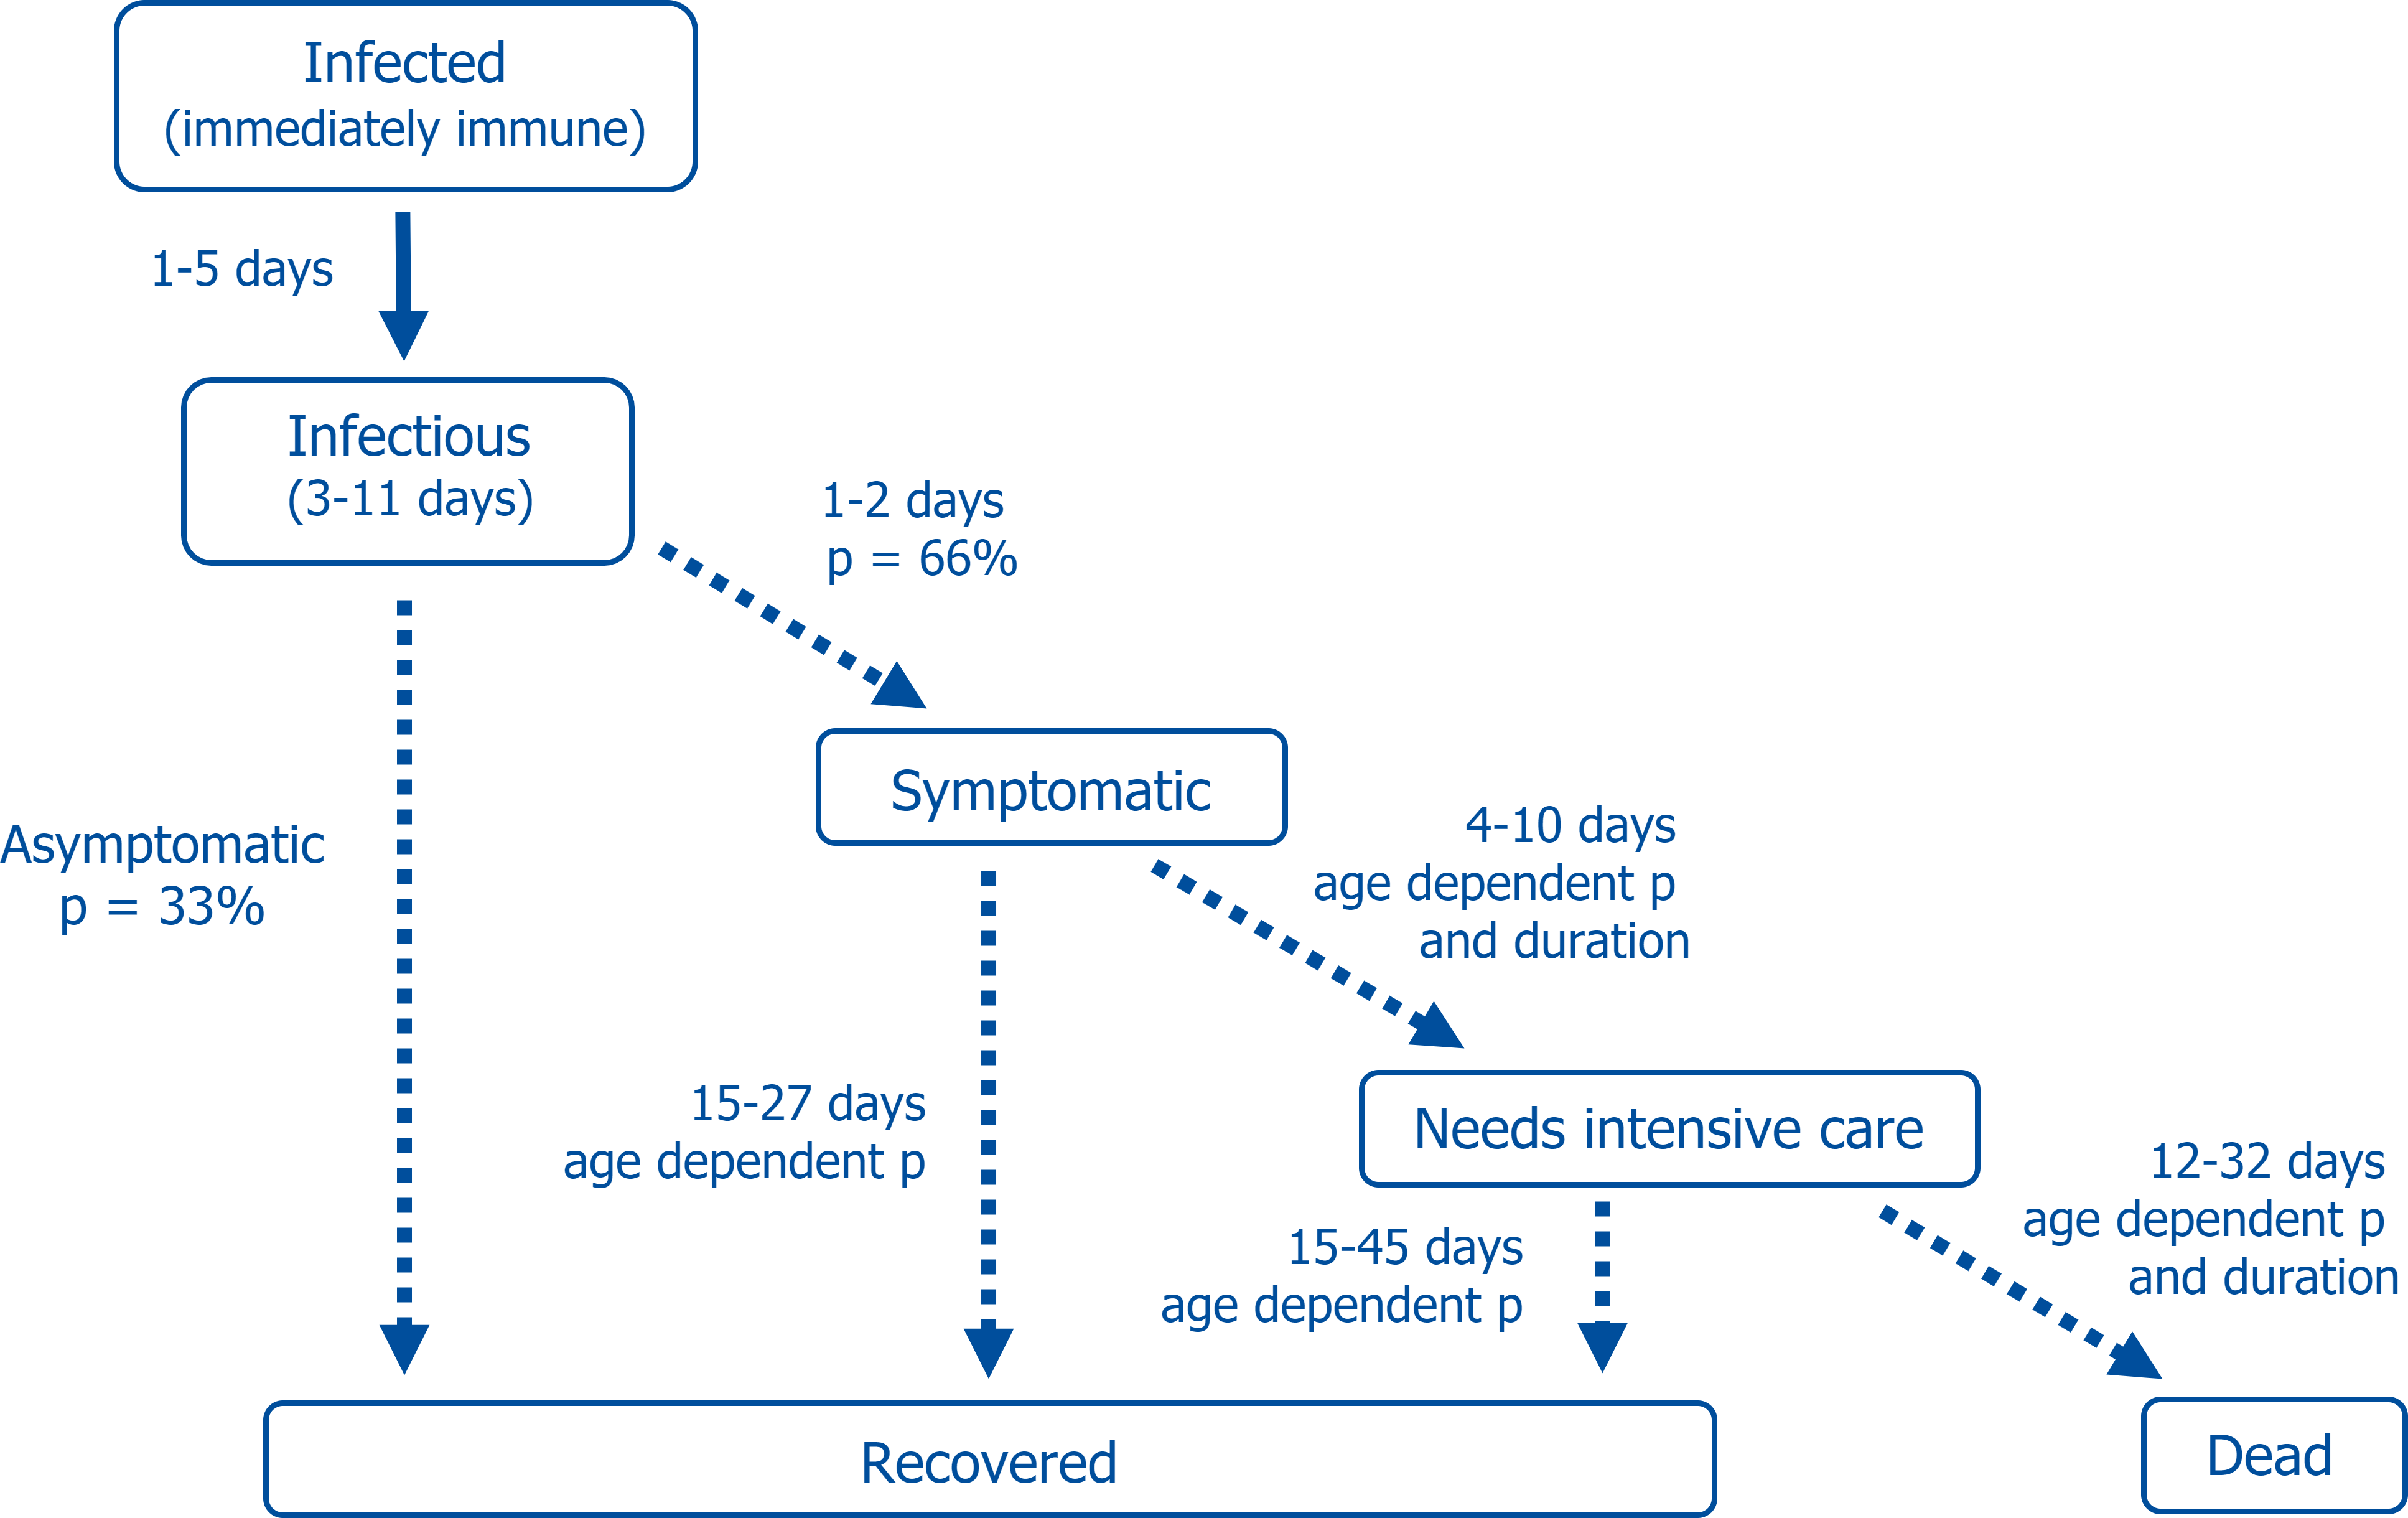
\includegraphics[width=\textwidth]{../figures/disease_progression.png}
    \caption{Course of Disease in the model}
    \label{fig:course_of_disease}
\end{figure}

First, infected individuals will become infectious after one to five days. About one third of people stays asymptomatic. The rest develops symptoms about one to two days after they become infectious. Modeling asymptomatic and pre-symptomatic cases is important because those people do not reduce their contacts or demand a test and can potentially infect many other people \citep{Donsimoni2020}.

A small share of symptomatic people will develop strong symptoms that require intensive care. The exact share and time span is age-dependent. An age-dependent share of intensive care unit (ICU) patients will die after spending up to 32 days in intensive care. Moreover, if the ICU capacity was reached, all patients who require intensive care but do not receive it die.

It would be easy to make the course of disease even more fine-grained. For example, we could model people who require hospitalization but not intensive care. So far we opted against that because only the ICU capacity might become a bottleneck in Germany.

We allow the progression of the disease to be stochastic in two ways: Firstly, state changes only occur with a certain probability (e.g. only a fraction of infected individuals develops symptoms). Secondly, the number of periods for which an individual remains in a state is drawn randomly. The parameters that govern these processes are taken from the literature. They can vary with the age of an individual.

Detailed information on the calibration of the disease parameters is available as part of our \href{https://sid-dev.readthedocs.io/en/latest/reference_guides/epi_params.html}{online documentation}.
